\documentclass[12pt]{article}
\usepackage[margin=2cm]{geometry} 
\usepackage{amsmath,amsthm,amssymb,amsfonts,graphicx}
\usepackage[T2A]{fontenc}
\usepackage[utf8]{inputenc}
\usepackage[english, russian]{babel}
\usepackage[export]{adjustbox}
\usepackage{listings}

\begin{document}
\title{
	Волновая динамика \\
	Отчёт
}
\author{Бредихин Никита}
\date{}
\maketitle

\section{Постановка задачи}
Рассматривается плоская волна в двухмерном пространстве. Плоская волна является частным решением волнового уравнения. Такая волна в природе не существует, так как фронт плоской волны начинается в $-\infty$ и заканчивается в $+\infty$, чего, очевидно, быть не может. Кроме того, плоская волна переносила бы бесконечную мощность, и на создание плоской волны потребовалась бы бесконечная энергия.

Необходимо визуализировать данную математическую модель и получить наглядное изображение плоской волны.
\section{Описание модели}
Уравнение любой волны является решением дифференциального уравнения, называемого волновым. Волновое уравнение для функции A записывается в виде
$$
	\Delta A(\vec{r},t) = \frac {1} {v^2} \, \frac {\partial^2 A(\vec{r},t)} {\partial t^2} \
$$

В общем виде уравнение плоской волны записывается следующим образом:
\begin{equation}
\label{wave_eq}
	\xi = A\cos\omega\left(t-\frac{x}{\nu}\right),
\end{equation}
где $\xi$ - смещение любой из точек с координатой $x$ в данный момент времени $t$, $A$ - амплитуда, $\omega$ - частота волны.

\section{Выполнение задачи}
Для получения наиболее наглядных результатов, в качестве основы для выполнения задачи был использован \textbf{JavaScript}. С помощью данной технологии удалось создать визуализацию эксперимента, которая может работать во всех современных веб-браузерах.

Волна отображается в виде сетки, для каждой точки которой смещение рассчитывается по формуле \eqref{wave_eq}. Далее формула \eqref{wave_eq} была модифицирована следующим образом:
\begin{equation}
\label{wave_eq}
	\xi = A\cos\omega\left(t-\frac{x}{\nu}\right) \exp(-t)
\end{equation}
Это позволило получить изображение для затухающей с течением времени волны.

Далее программа была модифицирована таким образом, чтобы время отсчитывалось отдельно для каждого слоя по оси $x$. Это позволило изобразить перемещение фронта волны.

\begin{figure}[ht]
	\label{fig:pic1}
	\caption{Затухающая волна}
	\centering
		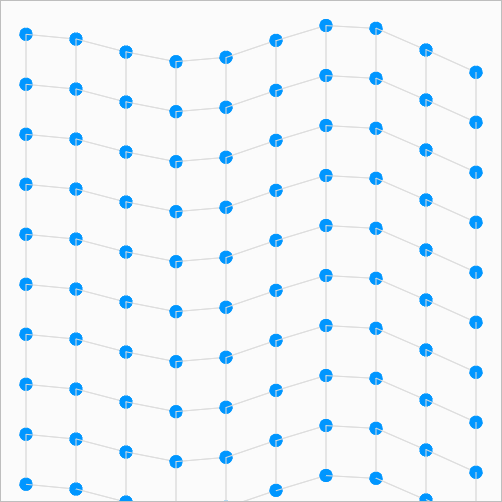
\includegraphics[width=0.5\columnwidth]{wd.png}
\end{figure}

\begin{figure}[ht]
	\label{fig:pic2}
	\caption{Движение фронта волны}
	\centering
		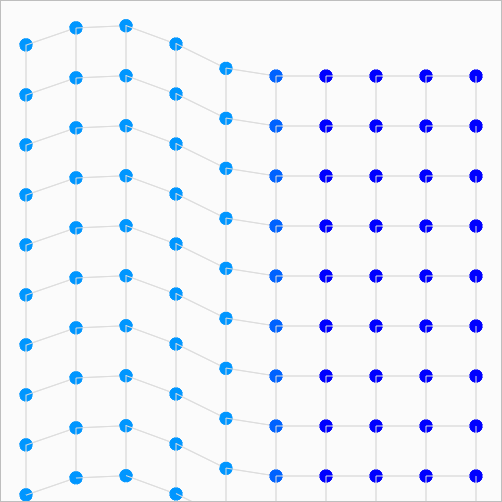
\includegraphics[width=0.5\columnwidth]{wd2.png}
\end{figure}
\end{document}